\newpage
\section{Setup and Simulation}
\subsection{Simulation using Lumerical FDTD}

The following simulation and calculation is aimed to reproduce the results of ref.~\cite{heeg} and is supposed to lead to a more accurate relation between local electromagnetic enhancement and total measured enhancement.

Lumerical FDTD is a commercial software to simulate the optical response of nanostructures using the FDTD method. Using this software the experimental setup of ref.~\cite{heeg} should be constructed inside the software to simulate the electromagnetic field around the gold nanostructure. The result of this simulation will be the enhancement of the electric field amplitude $\mathbf{E}(\mathbf{r})/E_0$ in three dimensional space. Compared to ref.~\cite{heeg} this will give a more detailed approximation of the spatial electromagnetic field than just a slice at the height of $z=40nm$ and allows at a later stage to calculate the enhancement along the graphene layer (see section~\ref{sec:calculations}).

\begin{figure}[!h]
  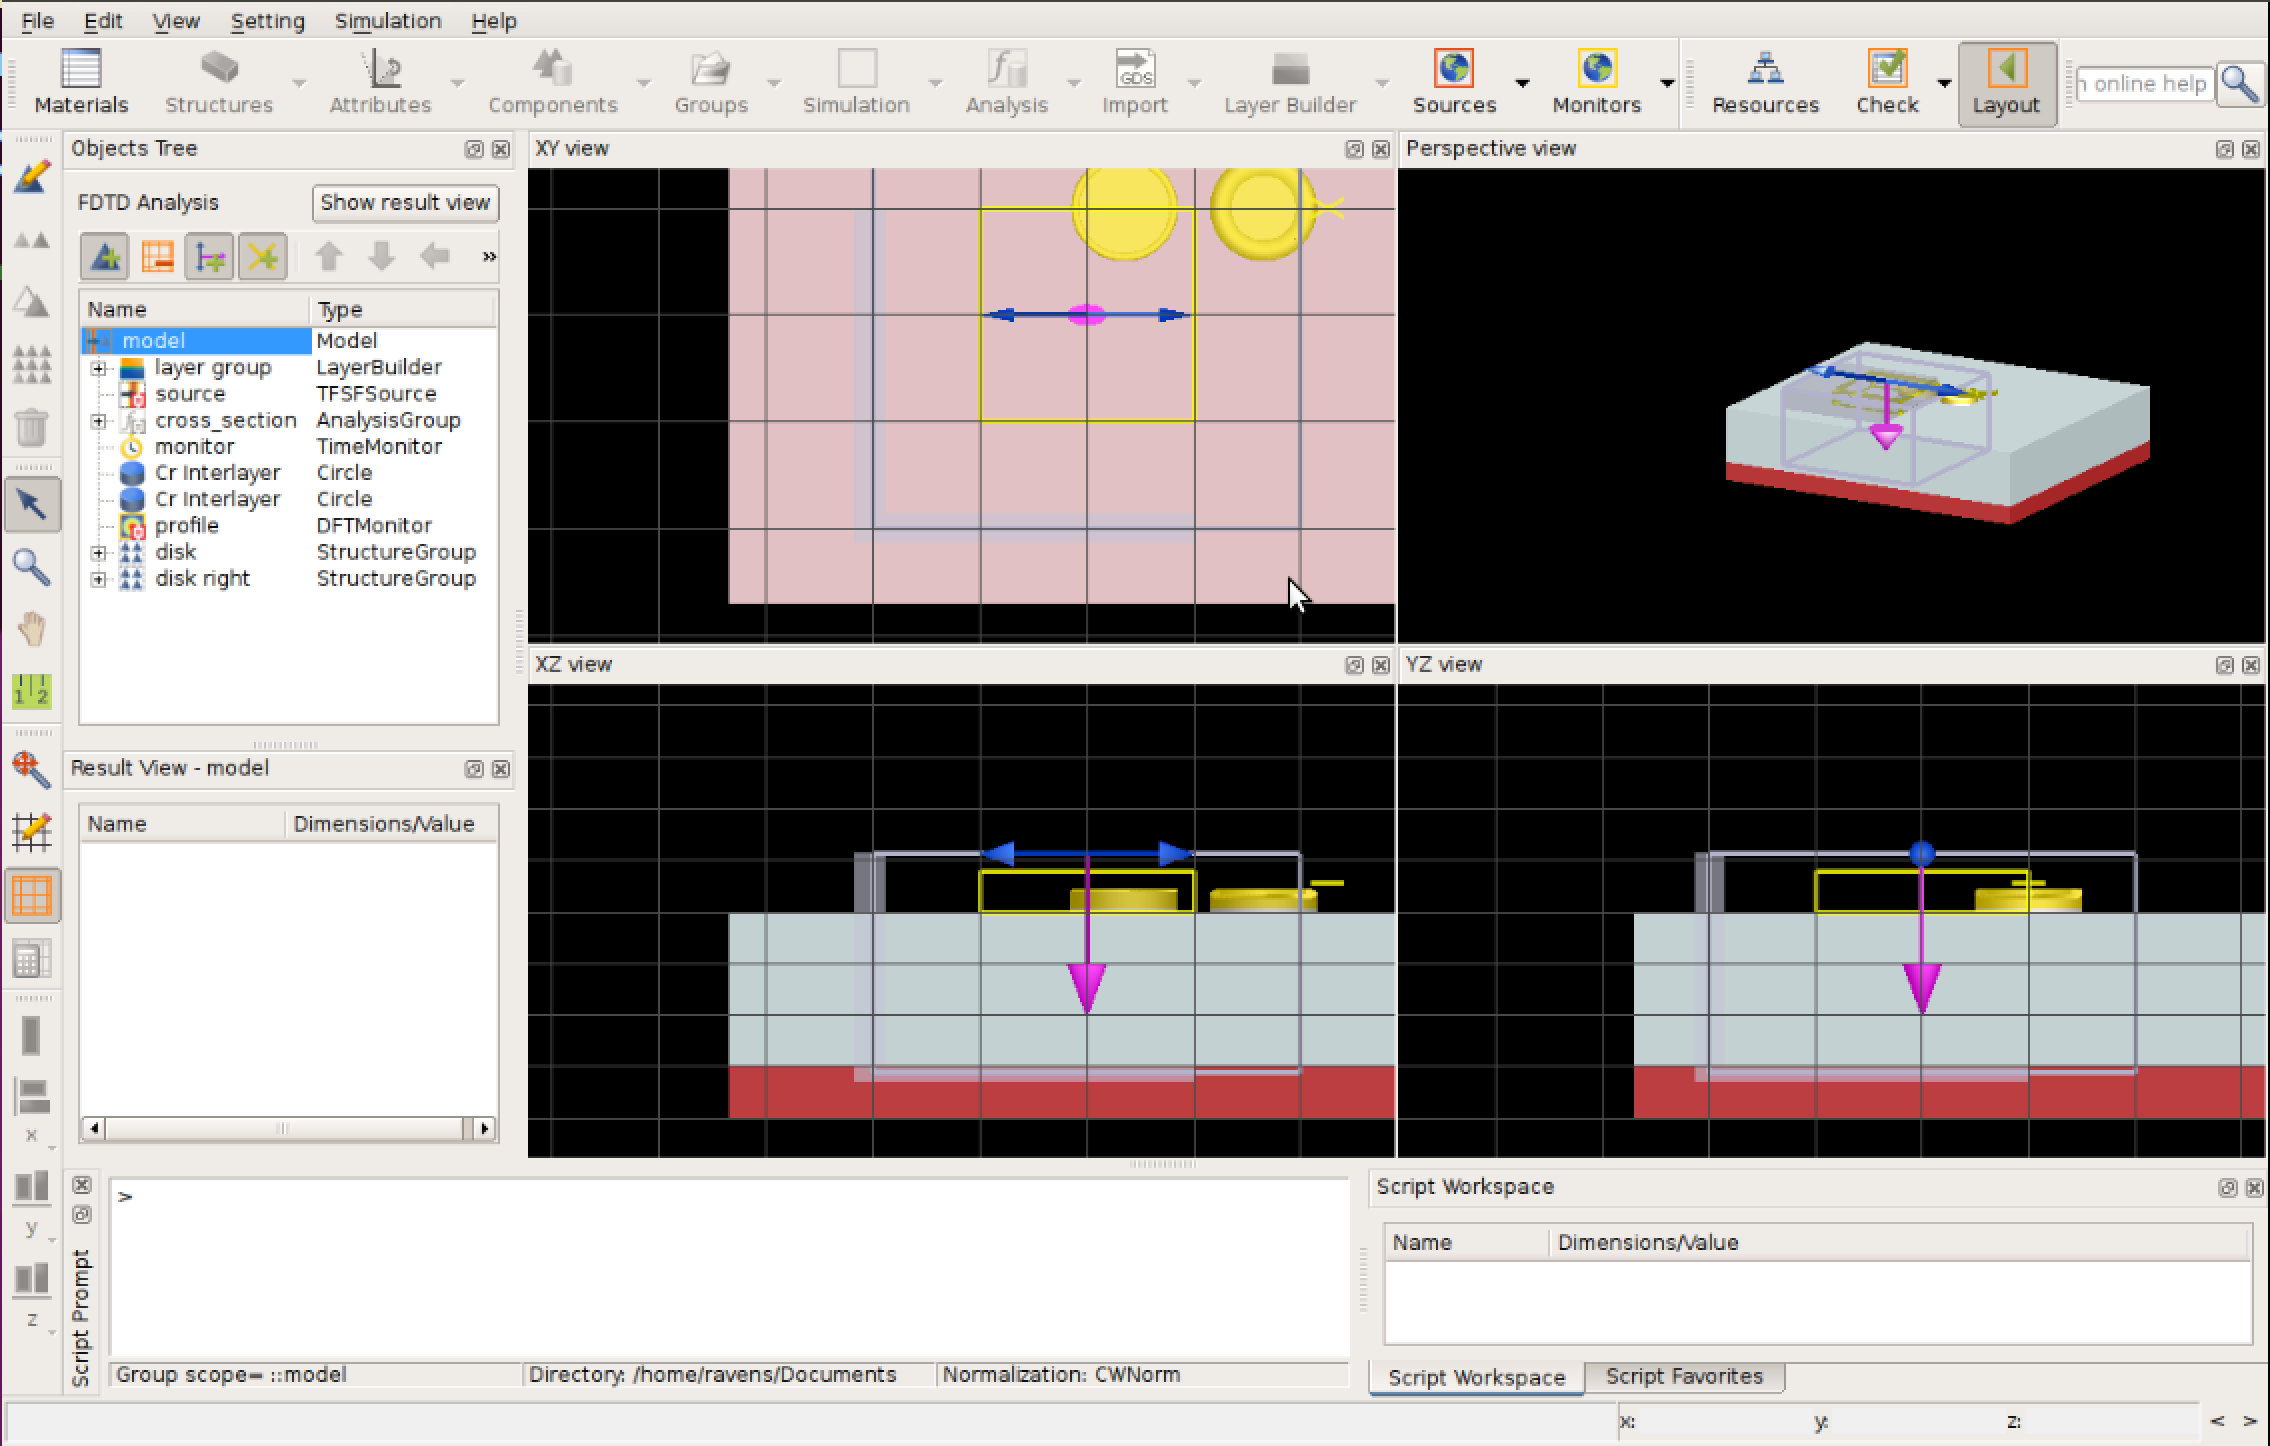
\includegraphics[width=\textwidth]{./images/lumerical.png}
  \caption{The experimental setup of ref.~\cite{heeg} simulated in Lumerical FDTD. Two gold disks with a radius of \SI{50}{nm} and a height of \SI{40}{nm} are placed \SI{30}{nm} apart with a \SI{5}{nm} Cr interlayer. They are placed on a Si substrate (red) with a \SI{300}{nm} SiO$_2$ layer (grey). The upper corners of the gold disks are rounded with a radius of \SI{2}{nm}. The simulation observes an area of $\SI{400}{nm}\times\SI{400}{nm}$ with a grid size of \SI{0.5}{nm}. To improve simulation time and memory consumption, only the lower left quarter (yellow box) is calculated and reproduced to the other quarters by using the mirror symmetry of the system. An incident plane wave with polarization along the dimer axis (blue arrows) and propagation towards the substrate (purple arrow) is assumed, using a total-field-scattered-field source (grey box).}
  \label{fig:lumerical}
\end{figure}

Lumerical allows to setup different materials in 3D space using basic geometric shapes like cubes, cylinders and spheres (figure~\ref{fig:lumerical}). The base material of this experiment is a substrate layer of SiO$_2$ with a layer of Si below. On this layer there are two gold nanodisks of \SI{50}{nm} radius and \SI{40}{nm} height. These two discs are placed \SI{30}{nm} apart on the surface on top of a \SI{5}{nm} Cr interlayer. The setup is done via direct entry of positions and sizes of the geometric shapes to replicate the values of Figure 1c in ref.~\cite{heeg}.

The corner radius of the gold cylinders was not mentioned in ref.~\cite{heeg} The real nanostructure is not a perfect cylinder, therefore the simulations will be done subsequently with two different corner radii of \SI{2}{nm} and \SI{5}{nm}. Due to the spatial discretization no perfectly rounded corners but only rectangular approximations can be simulated. Such sharp corners can lead to high intensity features in the simulated near field.

By default the boundaries of an FDTD simulation are reflecting all magnetic and electric fields. In the experiment we observe a substrate surface that can be approximated as infinite compared to the length scale of the gold structure. To account for this the electric field leaving the simulated area is absorbed by a Perfectly Matched Layer (PML).

To save time during the FDTD simulation the mirror symmetry along the $x$ and $y$ axis is used. This reduces the required memory and time of the simulation by a factor of $\frac{3}{4}$ \note{(damit meine ich: nur ein viertel der eigentlichen ressourcen wird benötigt. passt das so?)}, leading to a significant improvement in iteration speed. Only the left bottom quarter of the experiment is simulated (see figure \ref{fig:lumerical}).

The grid size within the simulated area is set to a uniform equidistant grid with a mesh size of \SI{0.5}{nm} between the simulated points in $x$, $y$ and $z$ direction. The total simulated area on the bottom left is a square of \SI{200}{nm}, leading to a total calculateable square of \SI{400}{nm} after mirroring the simulated results. \note{Die PML Layer sind viel weiter weg. Das solltest du noch schreiben. Außerdem wurde adaptive-meshing verwendet und nur im Simulationsbereich so fein diskretisiert.}

The simulated light pulse is a femto second pulse with a wavelength of $\lambda=\SI{638}{nm}$, matching the resonance of the plasmonic antennas \cite{heeg}.

Simulating the described system took about 8 hours on the used machine and led to a file size of \SI{1.24}{GB} simulated data per simulation. This simulation was done for both a \SI{2}{nm} and a \SI{5}{nm} corner radius. Unless otherwise noted the following sections will use data from the \SI{2}{nm} simulation.

For an evaluation, the simulated data is exported to Matlab, including the three dimensional electric field (as complex values) and the three axes \note{Lumerical verwendet hier ein Rohdatenformat, die Skalierung, wo welche Achse liegt, wird separat gespeichert (und muss auch extra exportiert werden)}.

\begin{figure}[!h]
  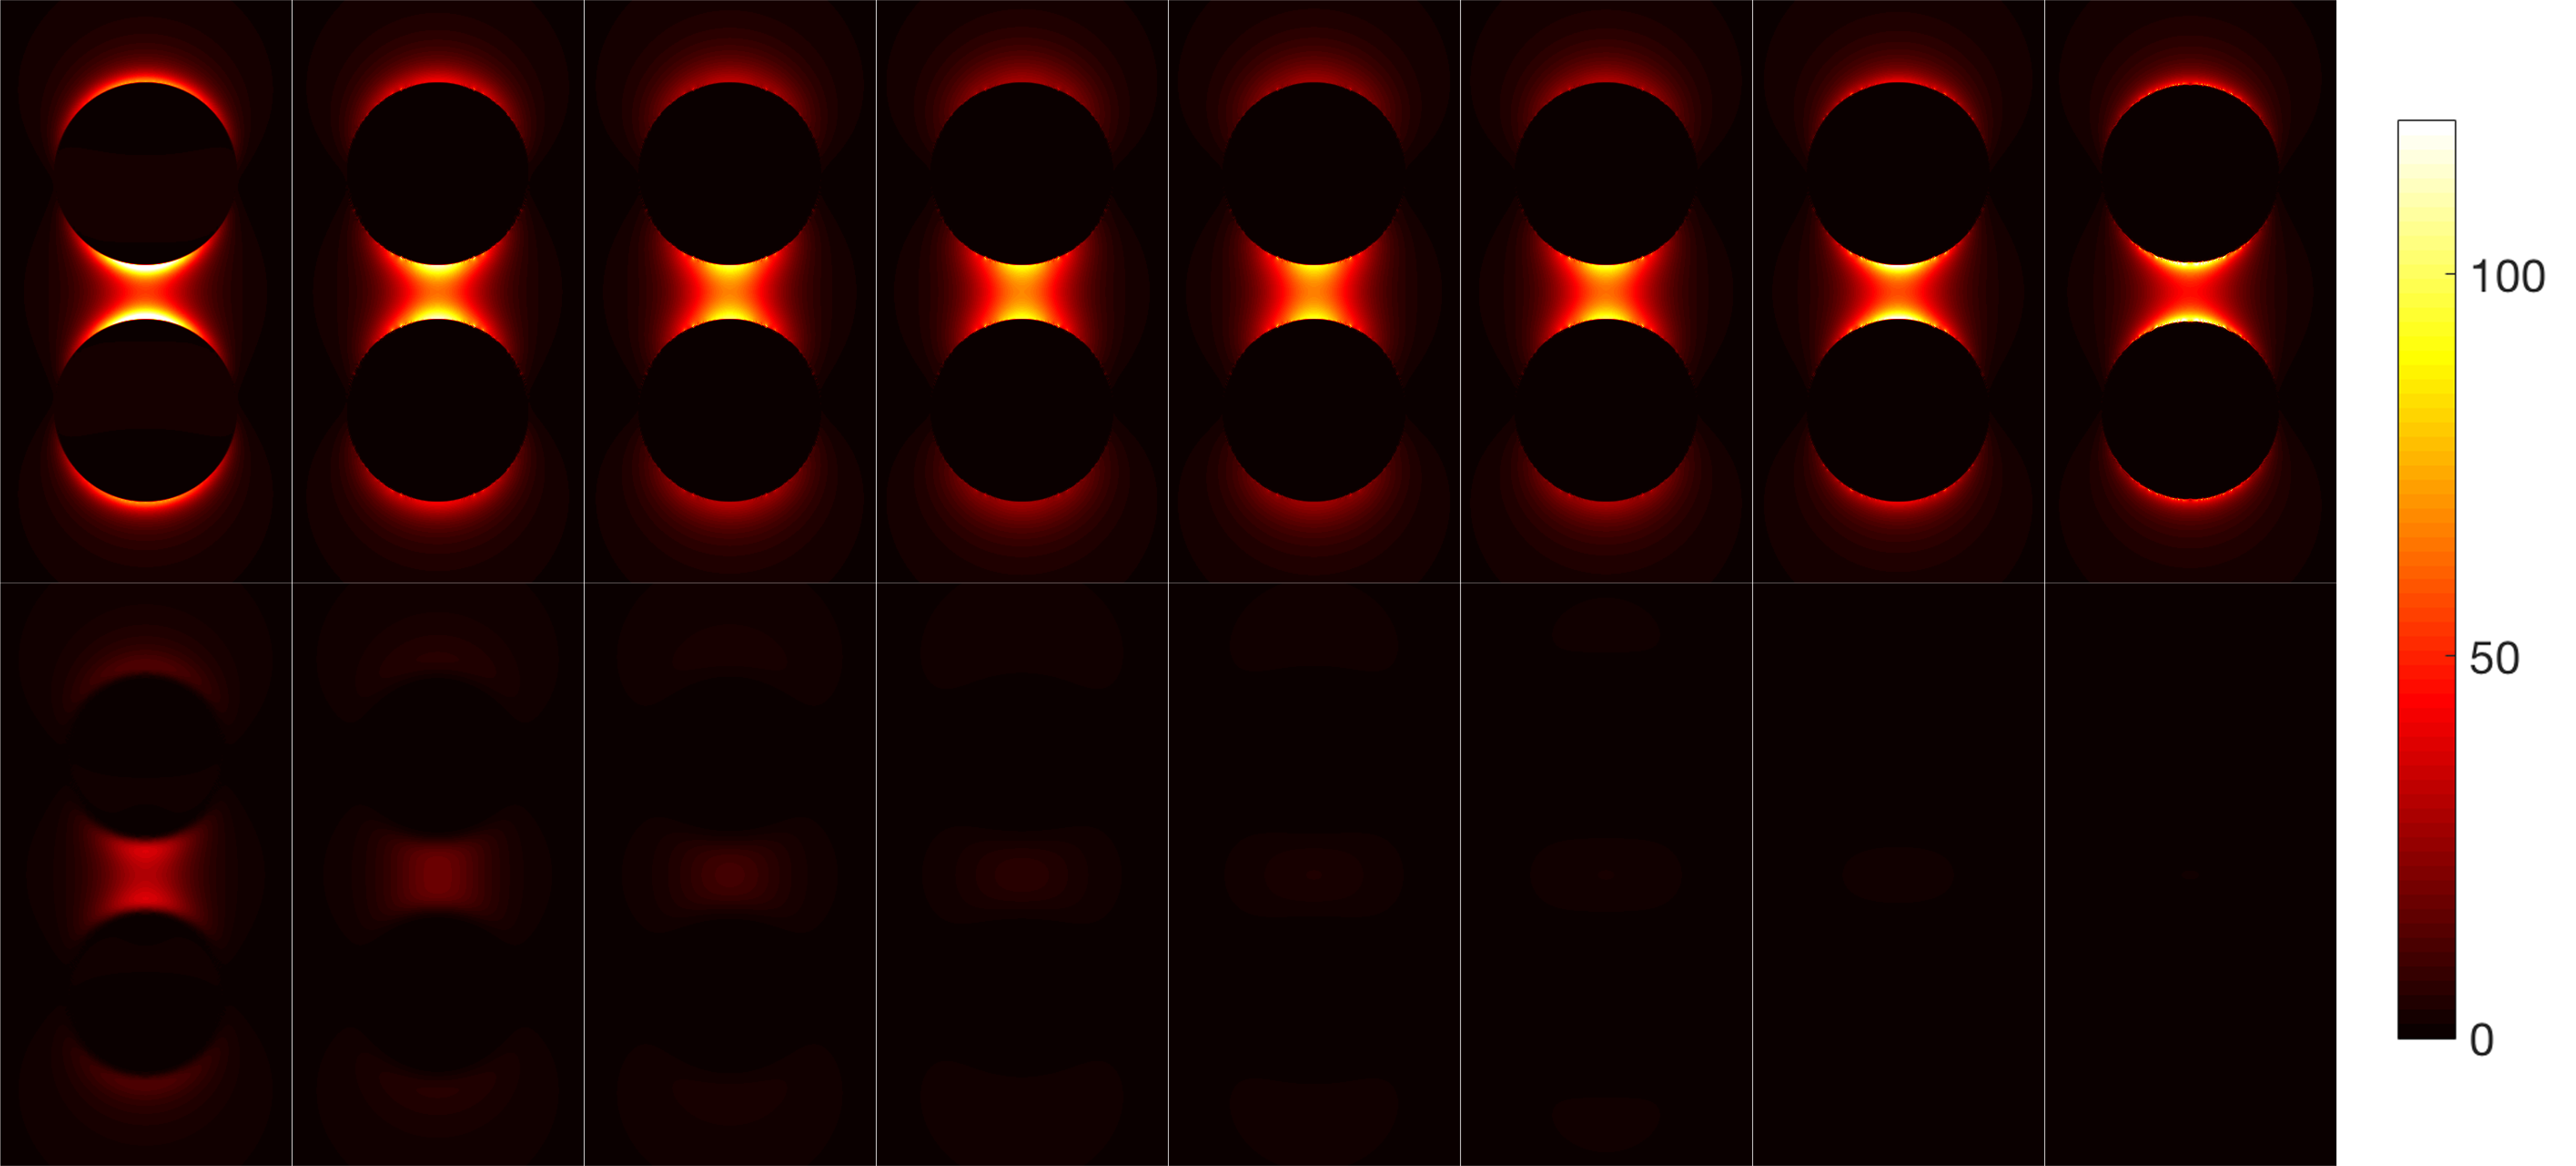
\includegraphics[width=\textwidth]{./images/simulation-slices.png}
  \caption{Slices of the simulation results in the $x y$-plane showing the near field enhancement $|E/E_0|^2$. Starting at the top left at $z=\SI{0}{nm}$ continuing in \SI{5}{nm} steps until $z=\SI{80}{nm}$. \note{Hier wäre eine Plotlegende hilfreich, die zeigt welche Farbe welcher Verstärkung entspricht. So wie in Fig. 13. Am besten auch noch die weißen Linien um die einzelnen Plots dicker machen.  Abbildung sollte später erscheinen.}}
  \label{fig:slices}
\end{figure}
